%%%%%%%%%%%%%%%%%%%%%%%%%%%%%%%%%%%%%%%%%
%
% CMPT 435
% Spring 2019
% Lab One
%
%%%%%%%%%%%%%%%%%%%%%%%%%%%%%%%%%%%%%%%%%

%%%%%%%%%%%%%%%%%%%%%%%%%%%%%%%%%%%%%%%%%
% Short Sectioned Assignment
% LaTeX Template
% Version 1.0 (5/5/12)
%
% This template has been downloaded from: http://www.LaTeXTemplates.com
% Original author: % Frits Wenneker (http://www.howtotex.com)
% License: CC BY-NC-SA 3.0 (http://creativecommons.org/licenses/by-nc-sa/3.0/)
% Modified by Alan G. Labouseur  - alan@labouseur.com
%
%%%%%%%%%%%%%%%%%%%%%%%%%%%%%%%%%%%%%%%%%

%----------------------------------------------------------------------------------------
%	PACKAGES AND OTHER DOCUMENT CONFIGURATIONS
%----------------------------------------------------------------------------------------

\documentclass[letterpaper, 10pt]{article} 


\usepackage[english]{babel} % English language/hyphenation
\usepackage[utf8]{inputenc}
\usepackage{graphicx}
\usepackage[lined,linesnumbered,commentsnumbered]{algorithm2e}
\usepackage{listings}
\usepackage{minted}
\usepackage{fancyhdr} % Custom headers and footers
\pagestyle{fancyplain} % Makes all pages in the document conform to the custom headers and footers
\usepackage[table]{xcolor}
\usepackage{csquotes}
\usepackage{natbib}
\usepackage[nottoc]{tocbibind}
\usepackage{lastpage}
\usepackage{url}
\usepackage{float}
\usepackage{scrextend}
\usepackage{epigraph}
\fancyhead{} % No page header - if you want one, create it in the same way as the footers below
\fancyfoot[L]{} % Empty left footer
\fancyfoot[C]{page \thepage\ of \pageref{LastPage}} % Page numbering for center footer
\fancyfoot[R]{}
\usepackage{listings}% http://ctan.org/pkg/listings
\usepackage{hyperref}
\renewcommand{\headrulewidth}{0pt} % Remove header underlines
\renewcommand{\footrulewidth}{0pt} % Remove footer underlines
\setlength{\headheight}{13.6pt} % Customize the height of the header
\usepackage{pgfplots}
\pgfplotsset{width=7cm,compat=1.8}

%----------------------------------------------------------------------------------------
%	TITLE SECTION
%----------------------------------------------------------------------------------------

\newcommand{\horrule}[1]{\rule{\linewidth}{#1}} % Create horizontal rule command with 1 argument of height

\title{	
   \normalfont \normalsize 
   \textsc{CMPT 435 - Fall 2020 - Dr. Labouseur} \\[10pt] % Header stuff.
   \horrule{0.5pt} \\[0.25cm] 	% Top horizontal rule
   \large{Assignment Two -- Sorting Algorithms} \\
   \textsc{Applying Sorting Algorithms to a list of Strings}\\[20pt]% Assignment title

   \horrule{0.5pt} \\ 	% Bottom horizontal rule
   


	% Today's date.
   \author{Sam Alcosser \\ \normalsize Samuel.Alcosser1@Marist.edu}
\date{\normalsize\today} 
}
\begin{document}




\fontfamily{bch}\selectfont
\maketitle
\tableofcontents
\newpage

\section{Introduction}

This document describes four different methods for sorting items, and implementations of those methods, or algorithms, in C++. The four methods are known as insertion sort, selection sort,  merge sort, and quick sort. Merge sort and quick sort are more efficient as they implement recursion within their sorting processes, as seen in the chart above. The reason for this will be discussed later on.

\section{Ontology of the \texttt{Sort} class}

The \texttt{Sort} class seen below contains all of the different sorts as static functions, with the idea that the main running function would then be able to have easy access to the methods. This class contains the sorting algorithms, helper functions such as \texttt{swap()} and \texttt{printList()}, and helper functions for the two recursive sorting algorithms.




\begin{addmargin}[-5em]{1em}
\begin{small}
\begin{minted}[linenos=true]{cpp}
#pragma once
#include <iostream>
#include <string>

class Sort {
public:


	static void swap(std::string &a, std::string &b);
	static void printList(std::string s[], int n);
	static int Insertion(std::string s[], int n);
	static int Selection(std::string s[], int n);
	static int subMSort(std::string s[], int l, int m, int r, int cnt);
	static void mergeSort(std::string s[], int lInd, int rInd, int &cnt);
	static void quickSort(std::string s[], int p, int r, int &cnt);
	static int Partition(std::string s[], int p, int r, int &cnt);

};

\end{minted}
\end{small}
\end{addmargin}



\vspace{1.5em}
\begin{center}
\textbf{A Quick Note}
\end{center}

To make sense of these algorithms, for each one I will start by giving an overview of the process including a diagram. After, I will show my implementation of the algorithm followed by a detailed description of each step with references to specific lines in the code. This is done to avoid the clutter of describing the algorithm itself and my implementation of said algorithm at the same time.

\section{Insertion Sort}
\subsection{Understanding Insertion Sort}
\begin{center}
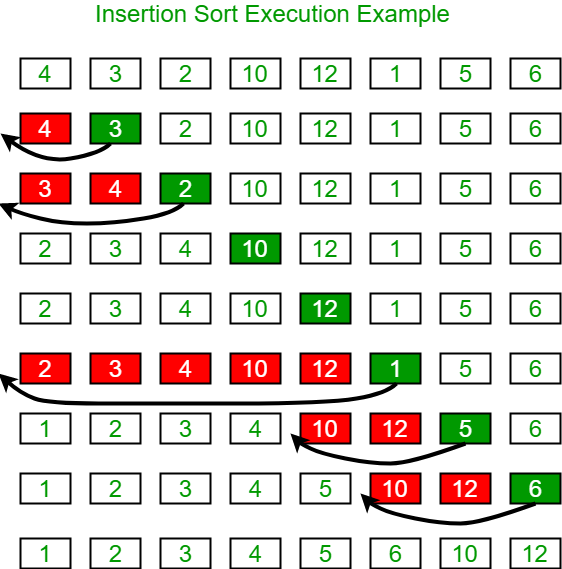
\includegraphics[width=\textwidth / 2]{img/insertionSort.png}
\end{center}
Insertion sort operates by stepping through each element of a list and comparing as it goes. Each current element will compare itself to each element that was before it in the order of the list, and swap. The site \textit{Programiz.com} has a better description of the method.


\begin{displayquote}
Insertion sort works similarly as we sort cards in our hand in a card game.

We assume that the first card is already sorted then, we select an unsorted card. If the unsorted card is greater than the card in hand, it is placed on the right otherwise, to the left. In the same way, other unsorted cards are taken and put at their right place.

A similar approach is used by insertion sort.

Insertion sort is a sorting algorithm that places an unsorted element at its suitable place in each iteration.
\end{displayquote}
{\textit{--programiz.com}}
\subsection{Implementation of Insertion Sort}

Insertion sort is probably the simplest of the sorting algorithms out of the four. This does not mean however that it is the most efficient, as will be evident later on. 







\begin{addmargin}[-5em]{1em}
\begin{small}
\begin{minted}[linenos=true]{cpp}



int Sort::Insertion(std::string s[], int n)
{
	int counter = 0;
	std::string last;
	for (int i = 1; i < n; i++)
	{
		last = s[i];
		int j = i - 1;
		while (j >= 0 && s[j] > last)
		{
			counter++;
			
			s[j + 1] = s[j];

			j = j - 1;
		}
	
		s[j + 1] = last;
	}

	//printList(s, n);		//debugging
	return counter;
}
\end{minted}
\end{small}
\end{addmargin}


\begin{center}
    \textbf{Code Breakdown}
\end{center}
\begin{enumerate}
    \item For each index in the array \texttt{s[]} after index one(Line 5)
    \item Compare the current element to the one before it (line 9)
    \item If the current element is smaller than the one before it, keep comparing until the current element is bigger than the next one being compared. At that point, shift all elements that were previously compared up by one. (lines 9-16)
    \item Place the current element in its place which was created by the movement of the other elements (line 18)
    \item Continue the same process until the end of the array.
\end{enumerate}

\newpage
\section{Selection Sort}
\subsection{Understanding Selection Sort}
\begin{center}
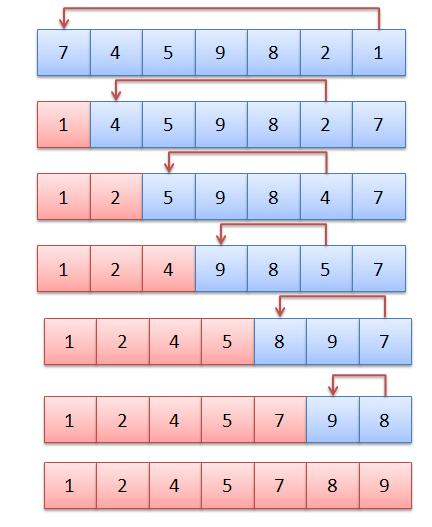
\includegraphics[width=\textwidth / 2]{img/SelectionSort.jpg}
\end{center}

Selection sort is a sorting algorithm similar to Insertion sort. Although, due to its differences, it is usually slower and less efficient. The process is quite simple. For every index in the array, if there is any value further in the array that is smaller than the current index, swap the current index with the lowest of those values.

\subsection{Implementation of Selection Sort}

The simplicity of selection sort can be seen below, as the total number of lines of code is even less than insertion sort.

\begin{addmargin}[-5em]{1em}
\begin{small}
\begin{minted}[linenos=true]{cpp}
int Sort::Selection(std::string s[], int n)
{
	int low;
	int counter = 0;
	for (int i = 0; i < n; i++)
	{
		low = i;
		for (int j = i + 1; j < n; j++)
		{
			counter++;

			if (s[j] < s[low])
			{
				low = j;
			}
		}
		Sort::swap(s[low], s[i]);
	}
	//printList(s, n);		//debugging
	return counter;
}
\end{minted}
\end{small}
\end{addmargin}

\begin{center}
    \textbf{Code Breakdown}
\end{center}

\begin{enumerate}
    \item for each element in the array \texttt{s[]} starting at index 0 (lines 5,6):
    \item Start by assuming that this current index \texttt{i} is the lowest value by assigning the index number to the \texttt{low} variable (line 7).
    \item For each element after \texttt{i}, compare it to element \texttt{s[low]} (lines 8-12)
    \item Whenever a lower element is found, mark that as the new lowest index (line 14). Now, all elements after this new element will be compared to the new lowest value, until the true lowest value is found.
    \item Once the inner iterator reaches the end of the array (line 8), swap the value of the current element \texttt{s[i]} with the newly found lowest element denoted by \texttt{s[low]} (line 17).
\end{enumerate}

\section{Merge Sort}
\subsection{Understanding Merge Sort}
\begin{center}
\textbf{Refresher on Recursion}
\end{center}

Before we progress any further, we should quickly refresh oursleves on the concept of recursion. Simply put, when a function is recursive, this means that it calls itself.




\begin{center}
\begin{small}
\begin{minted}[linenos=true]{py}
def fact(n):
	if n == 0:
		return 1
	else:
		return n * fact(n-1)

\end{minted}
\end{small}

\end{center}
The Python code above shows a simple use of recursion to calculate factorials. Since a factorial is just a number multiplied by each integer below it in succession, this can be expedited by recursion. Notice how on line 5 the function calls itself by passing \texttt{n-1} to itself. With this, the function can continue. The next part of recursion is its base case of 0. Without this, the program will never finish, and possibly will cause a stack overflow error. By having a base case, there is a breakpoint for the code where it will begin to move back up the chain of calculation, freeing up the stack as it progresses.







\begin{center}
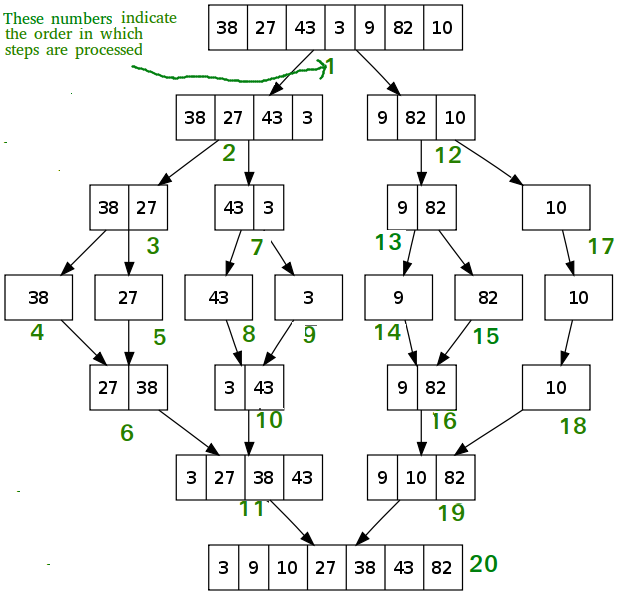
\includegraphics[width=\textwidth]{img/MergeSort.png}
\end{center}

Upon first glance of the graphic above, one may think that merge sort is much more complex than the previous two algorithms discussed. This person would be correct. Although, it is easier to understand after it is broken into its parts. These parts being the splitting, and the sorting. To begin, we will discuss the splitting function, which also happens to be the recursive function.

\subsection{Implementation of Merge Sort}
\begin{addmargin}[-5em]{1em}
\begin{small}
\begin{minted}[linenos=true]{cpp}
void Sort::mergeSort(std::string s[], int lInd, int rInd, int &cnt)
{

	int m = 0;

	if (lInd < rInd)
	{
		m = lInd + (rInd - lInd) / 2;
		mergeSort(s, lInd, m, cnt);
		mergeSort(s, (m + 1), rInd, cnt);

		cnt += Sort::subMSort(s, lInd, m, rInd, cnt);
	}
	else
	{
		//int n = sizeof(*s) / sizeof(s[0]);
		//printList(s, n);
	}
}


\end{minted}
\end{small}
\end{addmargin}


\begin{center}
\textbf{Unforeseen Issues}
\end{center}

Up until now, I have not acknowledged the lines of code dedicated to counting comparisons, because they are not integral to the function of the algorithms. In this sorting method though, it was a particular challenge. The reason being that this function is recursive, and therefore I could not simply run the function, count the comparisons as it goes, and then return it. Because of this, in this algorithm along with Quick Sort, I passed a reference to a count variable I called \texttt{cnt}.  This way I could have the algorithms increment the counter while not having to worry about maintaining the variable within themselves. Now on to the description.
\begin{center}
    \textbf{Code Breakdown}
\end{center}

\begin{enumerate}
     \item Check that there is actually enough range to sort by seeing if the left index is still before the right index (line 6)
      \item set \texttt{m}, our midpoint variable, to \texttt{lInd + (rInd - lInd) / 2}, in order to account for odd numbers (line 8).
    \item Call \texttt{mergeSort} on the first half (0-\texttt{m}) and the second half (\texttt{m+1} to end) (lines 9, 10) 
     \item Sort the array within the described bounds and add to the count (line 12).
\end{enumerate}

If the process still doesn't make sense, focus on the left and right indexes that are being passed to \texttt{mergeSort} on lines 9 and 10. 

\begin{center}
		\texttt{mergeSort(s, lInd, m, cnt);} \break
		\texttt{mergeSort(s, (m + 1), rInd, cnt);}
\end{center}

 Since this function will continue running until the left and right indexes match up, or when the bounds of the array given equal one index, these two lines will continue to take the given bounds and keep splitting them up into quarters, eighths, and so on until that base case is achieved. Now onto the sorting portion of the algorithm.
 
 \begin{addmargin}[-5em]{1em}
\begin{small}
\begin{minted}[linenos=true]{cpp}
int Sort::subMSort(std::string s[], int l, int m, int r, int cnt)
{
	int counter = 0;
	int len1 = m - l + 1;
	int len2 = r - m;

	std::string *left = new std::string[len1];
	std::string *right = new std::string[len2];

	for (int i = 0; i < len1; i++)
	{
		left[i] = s[l + i];
	}
	for (int j = 0; j < len2; j++)
	{
		right[j] = s[m + 1 + j];
	}
	int i = 0, j = 0;
	int k = l;
	while (i < len1 && j < len2) 
	{
		if (left[i] < right[j])
		{
			s[k++] = left[i++];
			counter++;
		}
		else
		{
			s[k++] = right[j++];
			counter++;
		}
	}
	while (i < len1)
	{
		s[k++] = left[i++];
	}
	while (j < len2)
	{
		s[k++] = right[j++];
	}
	return counter;
}

\end{minted}
\end{small}
\end{addmargin}

\begin{enumerate}
    \item Allocate space for the left side of the given portion of the array with the correct size (lines 4, 7).
    \item Allocate space for the right size of the given portion of the array with the correct size (lines 5, 8).
    \item Put the first half of the items in the given portion of the array to the \texttt{left} array, and the second half to the \texttt{right} array (lines 10-17)
    \item Set index counter \texttt{i} for the \texttt{left} array and \texttt{j} for the \texttt{right} array, both at 0. also set an index counter for the actual array as \texttt{k}, initiated with \texttt{l}, the left bound index for the array.(lines 18-19)
    \item Compare both the \texttt{left} and \texttt{right} arrays by index starting 0, whichever value at the current index is larger, place that value at the next index in the main array \texttt{s[]}. Increment the index counter on the sub array that the value was pulled from, as well as the index counter for the whole main array. This way, the sorting can continue (lines 20-32).
    \item Continue comparing until the end of either sub array is reached (line 20).
    \item At this point, append the remaining unsorted items after the last sorted index of \texttt{s[]} (lines 33-40).
    
   
\end{enumerate}


\section{Quick Sort}
\subsection{Understanding Quick Sort}
\begin{center}
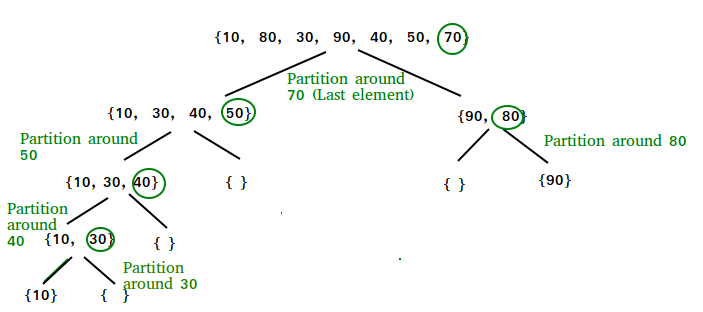
\includegraphics[width=\textwidth]{img/QuickSort.png}
\end{center}

Quick sort is even faster than merge sort. The reason being that much of the sorting is being done at the same time that the array is being broken up. This process will seem very similar to merge sort. Quick sort uses pivot values to choose where to compare values. The basic structure is to choose a pivot / partition value to start, and split at that point. Next, a new pivot value is chosen, and all values below the pivot value are put below the pivot value, and all values greater are put in front of the value. From here, a new pivot value is chosen and the process continues until each element is sorted in its place. The decision of what pivot value to use is widley discussed, although in my version I start with the last element.


\subsection{Implementation of Quick Sort}

Much like merge sort, quick sort calls itself recursivley on two halves of the given bounds. Although this time, the "midpoint" value is determined by the \texttt{partition} function.

 \begin{addmargin}[-5em]{1em}
\begin{small}
\begin{minted}[linenos=true]{cpp}
void Sort::quickSort(std::string s[], int p, int r, int &cnt)
{
	if (p < r)
	{
		int q = Sort::Partition(s, p, r, cnt);
		Sort::quickSort(s, p, (q - 1), cnt);
		Sort::quickSort(s, (q + 1), r, cnt);
	}
}


\end{minted}
\end{small}
\end{addmargin}

\begin{enumerate}
    \item Ensure that the given bounds account for more than one index (line 3)
    \item Use the \texttt{Partition()} function to sort the given bounds and return a new midpoint. (line 5)
    \item Call \texttt{quickSort()} on all elements from index 0 to \texttt{q} as defined by the \texttt{Partition} function.
\end{enumerate}

Below is the definition of the \texttt{Partition} function. It is most likely the most difficult to understand. At a very high level, it is placing elements in front of or behind the pivot element (chosen as the last element in the unsorted array) depending on if the value of the element is higher or lower than the pivot. Also, it returns the index of the next partition index.


 \begin{addmargin}[-5em]{1em}
\begin{small}
\begin{minted}[linenos=true]{cpp}
int Sort::Partition(std::string s[], int p, int r, int &cnt)
{
	std::string x = s[r];
	int i = p - 1;
	for (int j = p; j < (r - 1); j++)
	{
		if (s[j] <= x)
		{
			i++;
			cnt++;
			Sort::swap(s[i], s[j]);
		}else{
			cnt++;
		}
	}
	Sort::swap(s[(i + 1)], s[r]);
	return ++i;
}

\end{minted}
\end{small}
\end{addmargin}

\begin{enumerate}
    \item set the last element in the range as the pivot element \texttt{x} (line 3).
    \item variable \texttt{i}, used to point to the last sorted element below the pivot is initialized to \texttt{(p - 1)}(line 4).
    \item begin an for loop with an iterator called \texttt{j}. Initiate \texttt{j} with p and continue until \texttt{(r - 1)} (line 5).
    \item If value \texttt{s[j] <= x}, then increment \texttt{i},  and swap the values \texttt{s[i]} and \texttt{s[j]} (lines 7-12)
    \item After exiting the for loop, swap \texttt{s[(i + 1)]} and \texttt{s[r]}.(line 16)
    \item Finally, \texttt{Partition} returns \texttt{i} after incrementing it one final time. With this, the \texttt{Partition} function returns the new pivot index (line 17).
    \end{enumerate}







\section{Setup and Execution}

Finally, Here is a brief description of the actual execution of these algorithms. 
 \begin{addmargin}[-5em]{1em}
\begin{small}
\begin{minted}[linenos=true]{cpp}
const int len = 666; //normal mode  finishes in ~15 - 35 ms

std::string arr[4][len];
//std::string arr[len];
void setup()
{
...
...
...
				arr[i][count++] = ln;
...
...
...
}
\end{minted}
\end{small}
\end{addmargin}

I have excluded most of the \texttt{setup()} function, as it is a direct copy from the \texttt{AlanParse()} function. Briefly, it reads in the .txt file line by line to an array for use by the functions. The only difference this time is that the list needs to be reused. In the beginning, this was done by using a function called \texttt{reset()} to erase all of the content from the array each time. This was used between executions of the different algorithms.

Although When playing around with multithreading (which never was completed) I realized that I could not have just one array. The reason being that there would be memory issues if four separate threads were accessing the same memory. So, on line 10, it is clear to see that I made a multidimensional 4x666 array of strings. Each subarray for each algorithm. Although the dream of having multithreading, and testing on greater numbers of strings was never realized, this was a much cleaner organization of the data.



 \begin{addmargin}[-5em]{1em}
\begin{small}
\begin{minted}[linenos=true]{cpp}
int main()
{
	setup();
	std::cout << "Insertion sort made " << std::to_string(Sort::Insertion(arr[0], len)) << " comparisons." << std::endl;

	std::cout << "Selection sort made " << std::to_string(Sort::Selection(arr[1], len)) << " comparisons." << std::endl;

	int cnt = 0;
	Sort::mergeSort(arr[2], 0, (len - 1), cnt);
	std::cout << "Merge sort made " << std::to_string(cnt) << " comparisons." << std::endl;

	int qCnt = 0;
	Sort::quickSort(arr[3], 1, len, qCnt);
	std::cout << "Quick sort made " << std::to_string(qCnt) << " comparisons." << std::endl;
	/* Sort::printList(arr[0], len); //test Insertion Sort
	Sort::printList(arr[1], len); //test Selection Sort
	Sort::printList(arr[2], len); //test Merge Sort
	Sort::printList(arr[3], len); //test Quick Sort */
}
\end{minted}
\end{small}
\end{addmargin}

The first to algorithms, insertion sort and selection sort, have nothing notable about their execution. They both are passed the array itself and the length of the array, and return an integer which is converted into a string to display. The execution of merge sort and quick sort are more complicated. Both are passed their array just as insertion and selection are, although these two get low and high bounds, as well as a count variable. As previously discussed, the bounds are very important to these sorts, as they are recursive. Without them, this process would be much more complicated.









\section{Conclusion: The Results}

Finally, the results tell the real story. It is clear to see that the recursion helped to make Merge Sort and Quick Sort considerably faster. This is easy to understand as both functions operate with $O((n)log(n))$ complexity. Logarithmic algorithms are much quicker already, as logarithms grow very slowly.
Compared to Selection sort and Insertion sort, their complexity of $O(n^2)$ stands no chance when it comes to speed. Although in the real world, this does not make much of a difference. On my personal laptop, a moderately powerful machine, I clocked the whole program to run in just around 30 milliseconds.

\begin{center}
{\rowcolors{2}{gray!50}{white!100}
 \begin{tabular}{||c c c c||} 
 \hline
 Sort & Comparisons \\ [0.5ex] 
 \hline\hline
 Insertion Sort& 114309 \\ 
 \hline
 Selection Sort& 221445 \\
 \hline
 Merge Sort& 5445 \\
 \hline
 Quick Sort& 7155 \\ [1ex] 
 \hline
\end{tabular}
}
\end{center}


\newpage
\textbf{Closing Thoughts}

 For someone not in the field of computer science, it may seem trivial to sort a list of numbers, or sentences, or anything else. Although to me, this was and still is one of the hardest things to grasp. Beyond that, this assignment began to get my wheels turning thinking about multi threading. I am sure that with more time, I would have had a working test case for  sorting over 1,000,000 items per algorithm, each being on a separate core. This can wait until the next assignment though.
 
{\textit{\color{red}\huge{\{S.A.\}}}}
\newpage
\section{Appendix}

\center\large\textbf{References}
\begin{small}

 \begin{lstlisting}[language=TeX]
 
Insertion Sort Algorithm, Programiz.com, www.programiz.com/dsa/insertion-sort. 

Insertion Sort, GeeksforGeeks, 25 July 2020, www.geeksforgeeks.org/insertion-sort/.

Merge Sort, GeeksForGeeks, 7 June 2020, www.geeksforgeeks.org/merge-sort/. 

Quick Sort, GeeksforGeeks, 4 Sept. 2020, www.geeksforgeeks.org/quick-sort/?ref=lbp. 

Selection Sort Algorithm, Top Sites, www.thetopsites.net/article/51681938.shtml. 
\end{lstlisting}

\textit{Used for Graphics and quotes}
\end{small}
\vspace{4em}

Another interesting metric is to compare the total lines of code per algorithm (in C++) compared to their number of comparisons. It should be noted that in this instance quick sort is less efficient than merge sort. This is truly down to the way that the pivot index is chosen. If the index was chosen at random, or some other way, the algorithm may be more efficient. 


\begin{center}
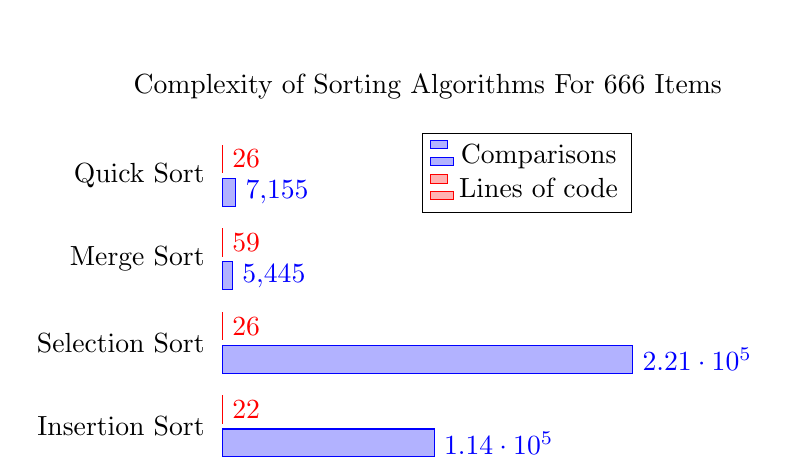
\begin{tikzpicture}
 \begin{axis}
[
    title    = Complexity of Sorting Algorithms For 666 Items,
    xbar,
    y axis line style = { opacity = 0 },
    axis x line       = none,
    tickwidth         = 0pt,
    enlarge y limits  = 0.2,
    enlarge x limits  = 0.02,
    nodes near coords,
    symbolic y coords = {Insertion Sort, Selection Sort,
                         Merge Sort, Quick Sort},
  ]
   \addplot coordinates { (114309,Insertion Sort) (221445,Selection Sort)
           (5445,Merge Sort) (7155,Quick Sort) };
            \addplot coordinates { (22,Insertion Sort) (26,Selection Sort)
           (59,Merge Sort) (26,Quick Sort)  };
             \legend{Comparisons, Lines of code}
               \end{axis}
               
\end{tikzpicture}
\end{center}

\end{document}
